\documentclass[conference]{IEEEtran}
\IEEEoverridecommandlockouts%
% The preceding line is only needed to identify funding in the first footnote. If that is unneeded, please comment it out.
\usepackage{cite}
\usepackage{amsmath,amssymb,amsfonts}
\usepackage{algorithmic}
\usepackage{graphicx}
\usepackage{textcomp}
\usepackage{xcolor}
\usepackage{float}
\usepackage{caption}
\usepackage{fancyhdr}
\usepackage{lastpage}

\captionsetup[figure]{name=Gambar}
\pagestyle{fancy}
\fancyhf{}
\fancyfoot[C]{\thepage}
\renewcommand{\headrulewidth}{0pt}
\renewcommand{\footrulewidth}{0.5pt}
% Ini adalah file utama




\def\BibTeX{{\rm B\kern-.05em{\sc i\kern-.025em b}\kern-.08em
    T\kern-.1667em\lower.7ex\hbox{E}\kern-.125emX}}
\begin{document}
\setcounter{page}{1}
\title{Analisis \textit{Fuzzy Time Series}: Mengungkap Pola Harga Singkong}

\author{\IEEEauthorblockN{1\textsuperscript{st} Agus Fuad Mudhofar}
\IEEEauthorblockA{\textit{Departemen Teknik Komputer} \\
\textit{Institut Teknologi Sepuluh Nopember}\\
Surabaya, Indonesia}
\and
\IEEEauthorblockN{2\textsuperscript{nd} Zadun Nafiq}
\IEEEauthorblockA{\textit{Departemen Teknik Komputer} \\
\textit{Institut Teknologi Sepuluh Nopember}\\
Surabaya, Indonesia}
\and
\IEEEauthorblockN{3\textsuperscript{rd} Daniel Oliver Enoch Bachtiar}
\IEEEauthorblockA{\textit{Departemen Teknik Komputer} \\
\textit{Institut Teknologi Sepuluh Nopember}\\
Surabaya, Indonesia}
\and
\IEEEauthorblockN{\hspace*{2.4cm}4\textsuperscript{th} Edrickson Edgar}
\IEEEauthorblockA{\hspace*{2.4cm}\textit{Departemen Teknik Komputer} \\
\hspace*{2.4cm}\textit{Institut Teknologi Sepuluh Nopember}\\
\hspace*{2.4cm}Surabaya, Indonesia}
\and
\IEEEauthorblockN{5\textsuperscript{th} Ahmad Aqbil Naim}
\IEEEauthorblockA{\textit{Departemen Teknik Komputer} \\
\textit{Institut Teknologi Sepuluh Nopember}\\
Surabaya, Indonesia}
}

\maketitle

\begin{abstract}
    Penelitian ini berfokus pada prediksi harga singkong di Indonesia menggunakan metode \textit{Fuzzy Time Series} (FTS). Harga singkong dipengaruhi oleh berbagai faktor seperti kondisi cuaca, permintaan pasar, kebijakan pemerintah, dan biaya produksi, yang dapat menyebabkan variabilitas harga dan berdampak pada pendapatan petani serta stabilitas ekonomi sektor pertanian. Data harga singkong bulanan dari tujuh provinsi di Indonesia selama periode 2020-2022 digunakan untuk membangun model FTS. Proses peramalan melibatkan beberapa langkah, yaitu menentukan interval data, memperoleh data historis, mendefinisikan \textit{fuzzy sets}, membangun hubungan logika \textit{fuzzy}, mencari pola hubungan antar data, dan melakukan peramalan. Hasil peramalan menunjukkan bahwa model FTS dapat memberikan estimasi harga singkong untuk bulan selanjutnya dengan tingkat kesalahan sebesar 2,45\% berdasarkan evaluasi menggunakan \textit{Mean Absolute Percentage Error} (MAPE). Model ini dapat digunakan sebagai alat bantu dalam perencanaan dan pengambilan keputusan di sektor pertanian, meskipun harus selalu diperbarui dengan data terbaru untuk meningkatkan akurasi.
\end{abstract}

\begin{IEEEkeywords}
\textit{Fuzzy Time Series}, Harga Singkong, Prediksi Harga
\end{IEEEkeywords}

\thispagestyle{fancy}
\fancyhf{}
\fancyfoot[C]{\thepage}
\renewcommand{\headrulewidth}{0pt}
\renewcommand{\footrulewidth}{0.5pt}
\section{Pendahuluan}
Indonesia merupakan salah satu negara yang sebagian besar penduduknya bermata pencaharian di bidang pertanian atau bercocok tanam [1]. Singkong merupakan salah satu komoditas pertanian yang memiliki peran penting dalam perekonomian banyak negara, termasuk Indonesia. Sebagai bahan pangan, singkong digunakan dalam berbagai produk makanan, pakan ternak, dan industri. Harga singkong dapat dipengaruhi oleh berbagai faktor seperti kondisi cuaca [2], permintaan pasar, kebijakan pemerintah, dan biaya produksi. Variabilitas harga ini tidak hanya mempengaruhi pendapatan petani tetapi juga berdampak pada stabilitas ekonomi di sektor pertanian. Selain itu, ketersediaan singkong yang luas di Indonesia menjadikan prediksi harga singkong penting untuk menjaga kesejahteraan sosial ekonomi masyarakat yang bergantung pada komoditas ini.

Dalam menghadapi tantangan ini, prediksi harga singkong dapat menjadi alat penting untuk memperkirakan harga beberapa bulan ke depan. \textit{Fuzzy Time Series} (FTS) adalah salah satu metode yang menawarkan keunggulan dalam memprediksi data berbasis waktu yang bersifat luas dan dapat digunakan dalam data \textit{realtime} [3]. Pendekatan FTS memungkinkan untuk menangkap ketidakpastian dan variabilitas data historis, memberikan prediksi yang lebih fleksibel dan adaptif terhadap perubahan kondisi. Penelitian ini bertujuan untuk mengungkap pola harga singkong menggunakan pendekatan Fuzzy Time Series dan mengembangkan model prediksi yang lebih akurat dan dapat diandalkan. Berdasarkan penelitianyang telah dilakukan oleh Widarma, A., \& Siregar, Y. H. (2020) dan Vatansever, M., Demir, İ., \& Hepşen, A. (2020)  fuzzy time series memiliki keunggulan dalam menangkap pola hubungan antar data yang bersifat fluktuatif dan tidak pasti, sehingga dapat memberikan prediksi yang lebih akurat dan andal.

Melalui analisis ini, penelitian ini tidak hanya berkontribusi pada pengembangan ilmu pengetahuan dalam bidang prediksi harga komoditas tetapi juga berpotensi meningkatkan stabilitas ekonomi sektor pertanian dengan menyediakan alat prediksi yang lebih efektif. Dengan demikian, teknologi FTS menawarkan solusi yang potensial untuk mengatasi fluktuasi harga singkong, sehingga mendukung kesejahteraan petani dan stabilitas ekonomi secara keseluruhan.


\section{Tinjauan Pustaka}

\subsection{\textit{Fuzzy Time Series}}
\textit{Fuzzy Time Series} (FTS) adalah metode peramalan yang pertama kali dikembangkan oleh Song dan Chissom pada tahun 1993 [4]. Mereka memperkenalkan FTS dalam upaya untuk memprediksi jumlah pendaftaran mahasiswa baru di Universitas Alabama. Sejak awal pengembangannya, FTS telah terbukti efektif dan fleksibel, sehingga diaplikasikan pada berbagai macam masalah peramalan lainnya. Beberapa contoh penerapan FTS termasuk peramalan penjualan, peramalan harga saham, dan peramalan tingkat polusi udara.

FTS menggunakan tiga prinsip utama dalam proses peramalan, yaitu Fuzzifikasi, Hubungan Logika Fuzzy (\textit{Fuzzy Logical Relationship}), dan Peramalan (\textit{Forecasting}). Fuzzifikasi adalah proses mengubah data numerik menjadi data \textit{fuzzy}, yaitu data yang diwakili oleh himpunan \textit{fuzzy}. Setelah data difuzzifikasi, langkah selanjutnya adalah membangun hubungan logika \textit{fuzzy}. Hubungan ini menggambarkan pola hubungan antar nilai data yang telah difuzzifikasi. Terakhir, berdasarkan hubungan logika \textit{fuzzy} yang telah dibangun, dilakukan peramalan untuk memprediksi nilai data di masa depan.

Secara lengkap, proses peramalan menggunakan FTS terdiri dari beberapa tahapan, yaitu:
    1) Memperoleh data historis (augmentasi data apabila diperlukan.)
    2) Menentukan interval data dan jumlah himpunan \textit{fuzzy}.
    3) Klasifikasi data.
    4) Mendefinisikan nilai FLRG (\textit{Fuzzy Logical Relationship Group}).
    5) \textit{Forecasting}.
    

\subsection{Prediksi Harga}
Prediksi harga adalah bidang penelitian yang sangat penting dalam ekonomi dan keuangan, karena memiliki implikasi langsung pada keputusan investasi, kebijakan moneter, dan strategi bisnis. Prediksi harga mencakup berbagai metode dan pendekatan, mulai dari metode statistik tradisional hingga teknik kecerdasan buatan yang lebih canggih [6].

Metode statistik tradisional seperti regresi linier, analisis deret waktu (time series), dan model autoregressive integrated moving average (ARIMA) telah lama digunakan untuk memprediksi harga. Regresi linier mencoba menemukan hubungan linear antara variabel prediktor dan harga. Misalnya, dalam pasar saham, faktor-faktor seperti pendapatan perusahaan, suku bunga, dan inflasi sering digunakan sebagai variabel prediktor untuk memodelkan harga saham [7]. Model ARIMA, di sisi lain, fokus pada pola dan tren dalam data historis harga untuk membuat prediksi [8]. Model ini menggabungkan komponen autoregressive (AR), differencing (I), dan moving average (MA) untuk menangkap dinamika data [9].

Selain itu, model berbasis teori himpunan fuzzy seperti fuzzy time series juga telah diterapkan dalam prediksi harga [10]. Metode ini memperhitungkan ketidakpastian dan ketidakjelasan dalam data, yang seringkali diabaikan oleh metode tradisional. Dalam fuzzy time series, data historis harga diubah menjadi himpunan fuzzy, dan aturan-aturan fuzzy diturunkan untuk meramalkan nilai di masa depan. Misalnya, studi oleh Song dan Chissom (1993) menunjukkan bahwa metode ini efektif untuk memprediksi data ekonomi yang bersifat fluktuatif dan tidak pasti [11].

Dalam literatur, terdapat banyak studi yang menunjukkan keberhasilan berbagai metode prediksi harga. Misalnya, studi oleh Zhang dan Wu (2009) membandingkan kinerja model ARIMA dengan jaringan saraf tiruan dalam memprediksi harga saham, dan menemukan bahwa jaringan saraf tiruan memberikan hasil yang lebih akurat [12]. Studi lainnya oleh Alptekin,D. dan Alptekin,B. (2017) memperkenalkan metode fuzzy time series yang diperbaiki untuk prediksi harga emas, menunjukkan bahwa pendekatan ini lebih unggul dibandingkan dengan metode prediksi tradisional dalam kondisi pasar yang bergejolak [13].

Secara keseluruhan, prediksi harga adalah bidang yang terus berkembang dengan berbagai pendekatan yang menawarkan keunggulan dan keterbatasannya masing-masing. Dengan kemajuan teknologi dan peningkatan kapasitas komputasi, diharapkan metode prediksi harga akan semakin canggih dan mampu memberikan hasil yang lebih akurat dan andal di masa depan.



\section{Metode Penelitian}

Penelitian ini menggunakan data harga singkong dari tahun 2020 hingga 2022 yang telah di augmentasi. Data ini diperoleh dari hasil laporan yang diterbitkan oleh Kementerian Pertanian Indonesia yang bekerja sama dengan Badan Pusat Statistik. Data yang digunakan adalah data bulanan yang mewakili banyak wilayah di Indonesia dengan didasarkan kepada 7 provinsi yaitu Lampung, Jawa Tengah, Jawa Timur, Jawa Barat, Sumatera Utara, Yogyakarta, dan NTT. Data ini kemudian diolah dan dianalisis menggunakan metode Fuzzy Time Series dengan diagram \textit{flowchart} sebagai berikut:

\begin{figure}[htbp]
    \centering
    {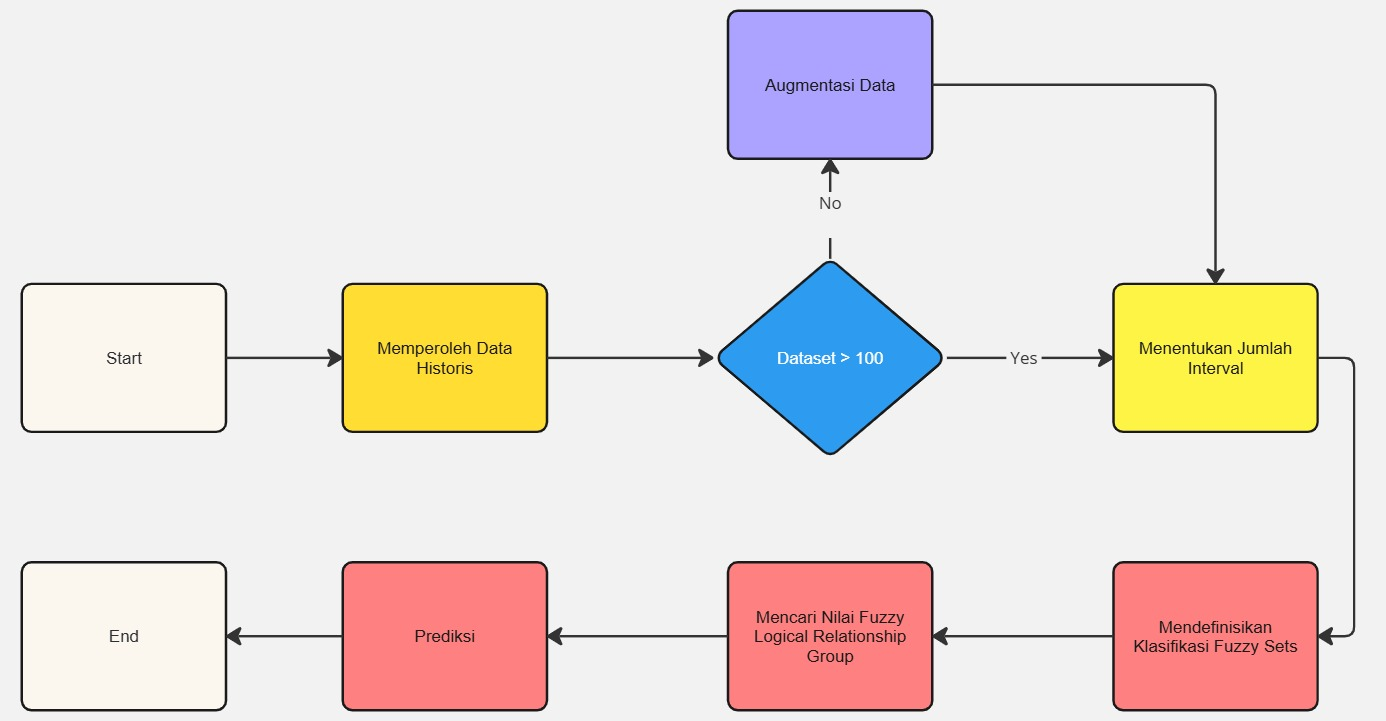
\includegraphics[scale=0.18]{images/Flowchart.jpg}} 
    \caption{\textit{Flowchart} Pengolahan Data}
\end{figure}


\subsection{Memperoleh Data Historis}
Data historis yang digunakan adalah data harga singkong dari tahun 2020 hingga 2022. Data ini diperoleh dari hasil laporan yang diterbitkan oleh Kementerian Pertanian Indonesia yang bekerja sama dengan Badan Pusat Statistik. Data yang digunakan adalah data bulanan yang mewakili banyak wilayah di Indonesia dengan didasarkan kepada 7 provinsi yaitu Lampung, Jawa Tengah, Jawa Timur, Jawa Barat, Sumatera Utara, Yogyakarta, dan NTT.

Data harga yang digunakan dalam penelitian ini adalah data harga singkong produsen dari tahun 2020 hingga 2022 yang telah dilakukan augmentasi. Data ini kemudian diolah dan dianalisis menggunakan metode Fuzzy Time Series untuk memprediksi harga singkong di bulan selanjutnya.

\subsection{Menentukan interval data dan jumlah himpunan \textit{fuzzy}}\label{AA}
Untuk menentukan interval data dan jumlah himpunan \textit{fuzzy} yang tepat, disini digunakan rumus Sturges sebagai berikut:

\begin{equation}
    k = 1 + 3.33 \times \log_{10}(n)
\end{equation}

Metode Sturges merupakan salah satu metode yang digunakan untuk menentukan jumlah kelas dalam distribusi data, yang kemudian dapat digunakan untuk menentukan jumlah himpunan \textit{fuzzy}. Rumus Sturges ini memperhitungkan ukuran sampel \( n \) dan memberikan aturan untuk menghitung jumlah kelas \( k \) sebagai fungsi logaritmik dari \( n \). Dalam konteks himpunan \textit{fuzzy}, jumlah kelas yang dihasilkan dari rumus Sturges dapat digunakan sebagai panduan untuk menentukan berapa banyak himpunan \textit{fuzzy} yang perlu dibuat untuk mencakup seluruh rentang data secara efektif. Pendekatan ini membantu dalam memastikan bahwa setiap himpunan \textit{fuzzy} memiliki interval yang tepat, sehingga memberikan representasi yang lebih akurat dari data yang dianalisis.

Secara praktis, metode Sturges sering digunakan karena kesederhanaannya dan kemampuannya untuk memberikan hasil yang cukup baik dalam berbagai situasi. Meskipun metode ini tidak selalu memberikan jumlah kelas yang optimal untuk semua jenis distribusi data, ia memberikan titik awal yang baik dan dapat disesuaikan lebih lanjut berdasarkan karakteristik spesifik dari data yang dianalisis. 

Dalam penerapan himpunan \textit{fuzzy}, penting untuk mempertimbangkan bahwa jumlah himpunan yang terlalu sedikit dapat mengaburkan detail penting, sedangkan jumlah yang terlalu banyak dapat membuat model menjadi terlalu kompleks dan sulit diinterpretasikan. Dengan demikian, metode Sturges memberikan keseimbangan yang baik antara kompleksitas dan keterwakilan data.



\subsection{Klasifikasi \textit{fuzzy sets}}
Dalam mendefinisikan \textit{fuzzy sets}, digunakan pengelompokkan berdasarkan interval data. Metode ini membagi data menjadi beberapa interval berdasarkan rentang nilai data. Setiap interval kemudian diwakili oleh sebuah \textit{fuzzy set} yang mencakup nilai-nilai dalam rentang tersebut. Dengan demikian, himpunan \textit{fuzzy} dapat memberikan representasi yang lebih fleksibel dan deskriptif dari data yang bersifat kontinu.

Selain menggunakan interval data, data historis juga berperan penting dalam menentukan batas-batas dan keanggotaan dari masing-masing \textit{fuzzy set}. Analisis data historis membantu dalam memahami distribusi dan pola data, sehingga interval dan fungsi keanggotaan \textit{fuzzy} dapat didefinisikan dengan lebih akurat. Pendekatan ini memastikan bahwa \textit{fuzzy sets} tidak hanya mencerminkan rentang nilai yang ada, tetapi juga memperhitungkan karakteristik statistik dan pola temporal yang terdapat dalam data historis.

% Membangun hubungan logika \textit{fuzzy}
\subsection{Mencari nilai FLRG}
Dalam membangun hubungan logika \textit{fuzzy}, digunakan metode Fuzzy Logical Relationship (FLR). Metode ini membangun hubungan antar data dengan menggunakan aturan \textit{fuzzy}. Aturan ini menggambarkan pola hubungan antar data yang telah difuzzifikasi. Metode ini akan memapping klasifikasi data harga bulan ini ke dalam klasifikasi data harga bulan selanjutnya. Dengan hasil mapping sebagai berikut:

Nilai FLRG adalah nilai yang didapat dari hasil mapping antara data harga bulan ini dengan data harga bulan selanjutnya. Nilai ini digunakan untuk memprediksi harga singkong di bulan selanjutnya.
Untuk mendapatkan nilai FLRG, digunakan rumus sebagai berikut:
    
\begin{equation}
        Nilai\; FLRG = \frac{\sum_{n=1}^{n_{th}} \text{Median (FLRG)}}{n_{th}}
    \end{equation}
    
\subsection{\textit{Forecasting}}
Langkah terakhir adalah memasukan data input kedalam model FTS dan melakukan peramalan. Dengan menggunakan data historis yang telah diperoleh, data input dimasukan kedalam model FTS. Model ini kemudian melakukan peramalan untuk memprediksi harga singkong di bulan selanjutnya. Hasil peramalan ini kemudian digunakan sebagai dasar untuk membuat keputusan yang lebih baik dalam merencanakan dan mengelola harga singkong. 

Dengan menggunakan model FTS, didapatkan hasil peramalan harga singkong untuk bulan selanjutnya. Hasil ini dapat menjadi perkiraan harga singkong di bulan selanjutnya. Peramalan harga singkong ini harus selalu diperbarui dengan data terbaru untuk mendapatkan hasil yang lebih akurat dan dapat diandalkan karena jika mengandalkan pola harga yang sudah lama, maka hasil peramalan akan kurang akurat.


\section{Hasil dan Pembahasan}

\subsection{Memperoleh data historis}
Data historis harga singkong digunakan sebagai dasar untuk analisis ini. Berikut adalah grafik yang menunjukkan data historis harga singkong:
\begin{figure}[H]
    \centering
    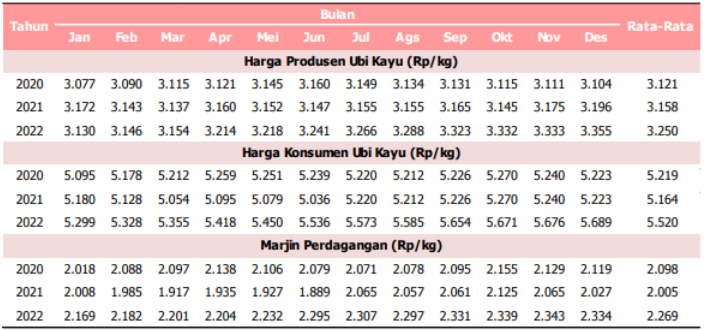
\includegraphics[scale=0.4]{images/Data Historis.png} 
    \caption{Data Historis Harga Singkong}
\end{figure}
Data tersebut kemudian diaugmentasi untuk memperoleh data yang lebih lengkap dan representatif. Karena data direkap bulanan, maka kode data augmentasi menggunakan tanggal untuk membedakan data asli dengan data augmentasi. Data augmentasi didapat dari penghitungan rata-rata bulan sebelumnya dan bulan setelahnya. Augmentasi dilakukan hingga data mencapai lebih dari 100 data. Data ini kemudian digunakan sebagai dasar untuk membangun model FTS.

\subsection{Menentukan interval data dan jumlah himpunan \textit{fuzzy}}

Untuk menentukan interval data dan jumlah himpunan \textit{fuzzy}, digunakan rumus Sturges. Berdasarkan rumus tersebut, data dibagi menjadi beberapa interval yang digunakan untuk menentukan jumlah himpunan \textit{fuzzy}. Menggunakan rumus Sturges, didapatkan jumlah himpunan \textit{fuzzy} sebanyak 8 interval data. Interval data ini kemudian digunakan sebagai dasar untuk membangun himpunan \textit{fuzzy} dan hubungan logika \textit{fuzzy}.



\subsection{Mendefinisikan \textit{fuzzy sets} berdasarkan interval data dan data historis}
Setiap interval kemudian diwakili oleh himpunan \textit{fuzzy}. Dalam penelitian ini, digunakan 8 interval data yang masing-masing diwakili oleh himpunan \textit{fuzzy}, yaitu:
\begin{figure}[H]
    \centering
    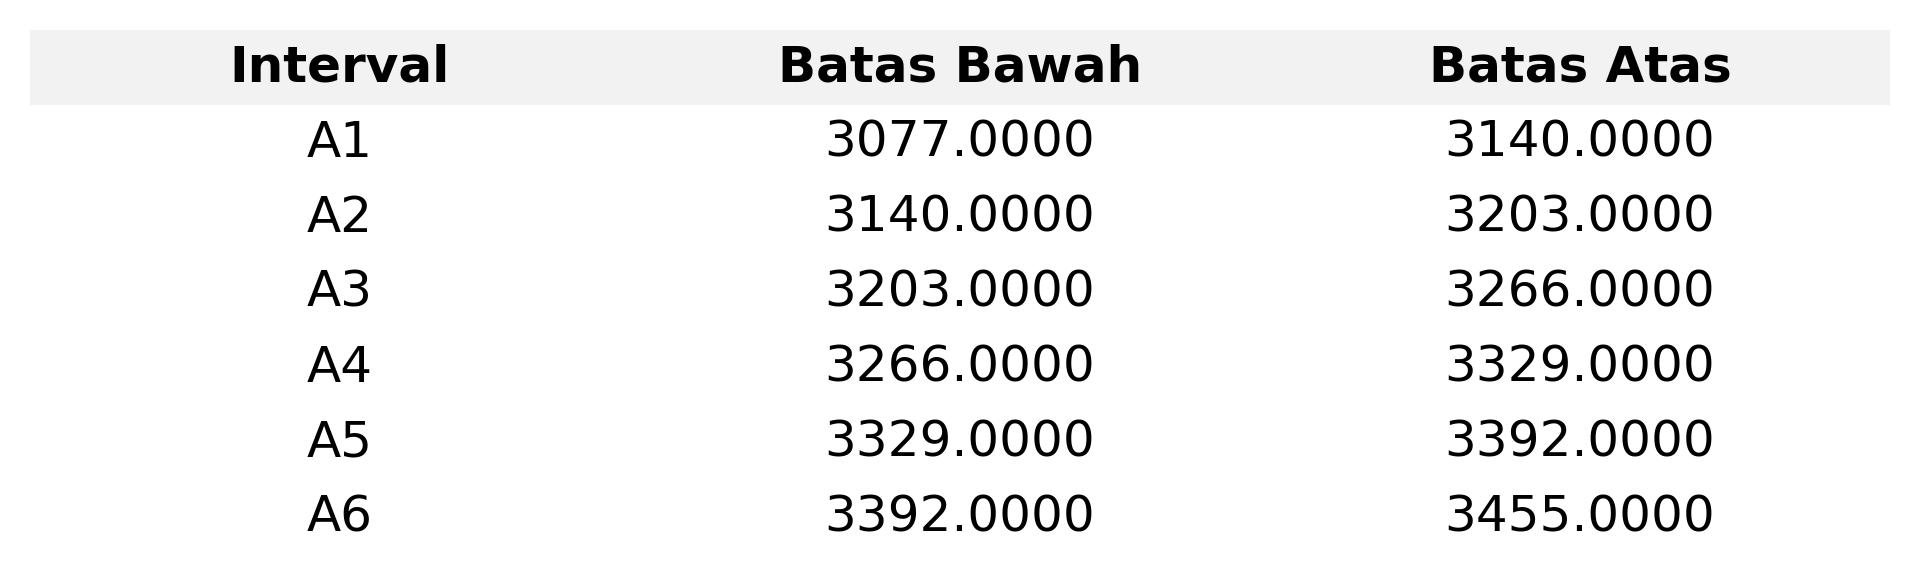
\includegraphics[scale=0.55]{images/intervals_table.jpg} 
    \caption{Fuzzifikasi data historis harga singkong}
\end{figure}

\subsection{Mencari nilai FLRG}
Setelah mendefinisikan \textit{fuzzy sets} berdasarkan interval data dan data historis, langkah selanjutnya adalah mencari nilai FLRG. Nilai FLRG didapat dengan cara memetakan klasifikasi data harga bulan ini ke dalam klasifikasi data harga bulan selanjutnya. Berikut adalah contoh hasil mapping data harga bulan ini ke data harga bulan selanjutnya:

\begin{figure}[H]
    \centering
    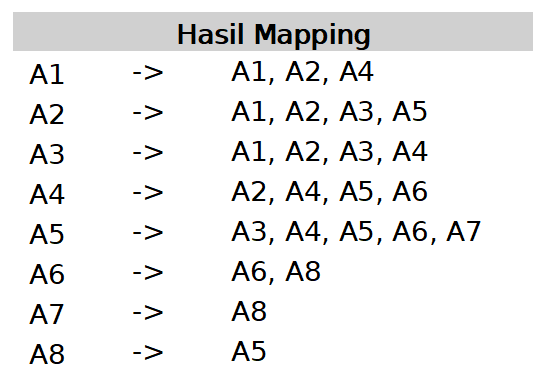
\includegraphics[scale=0.4]{images/hasil_mapping.png} 
    \caption{Pemetaan klasifikasi harga}
\end{figure}


Dari hasil pemetaan tersebut, didapatkan nilai FLRG yang digunakan untuk memprediksi harga singkong di bulan selanjutnya. Nilai FLRG ini merupakan hasil dari mapping antara data harga bulan ini dengan data harga bulan selanjutnya. Nilai ini kemudian digunakan sebagai dasar untuk memprediksi harga singkong di bulan selanjutnya.

\begin{figure}[H]
    \centering
    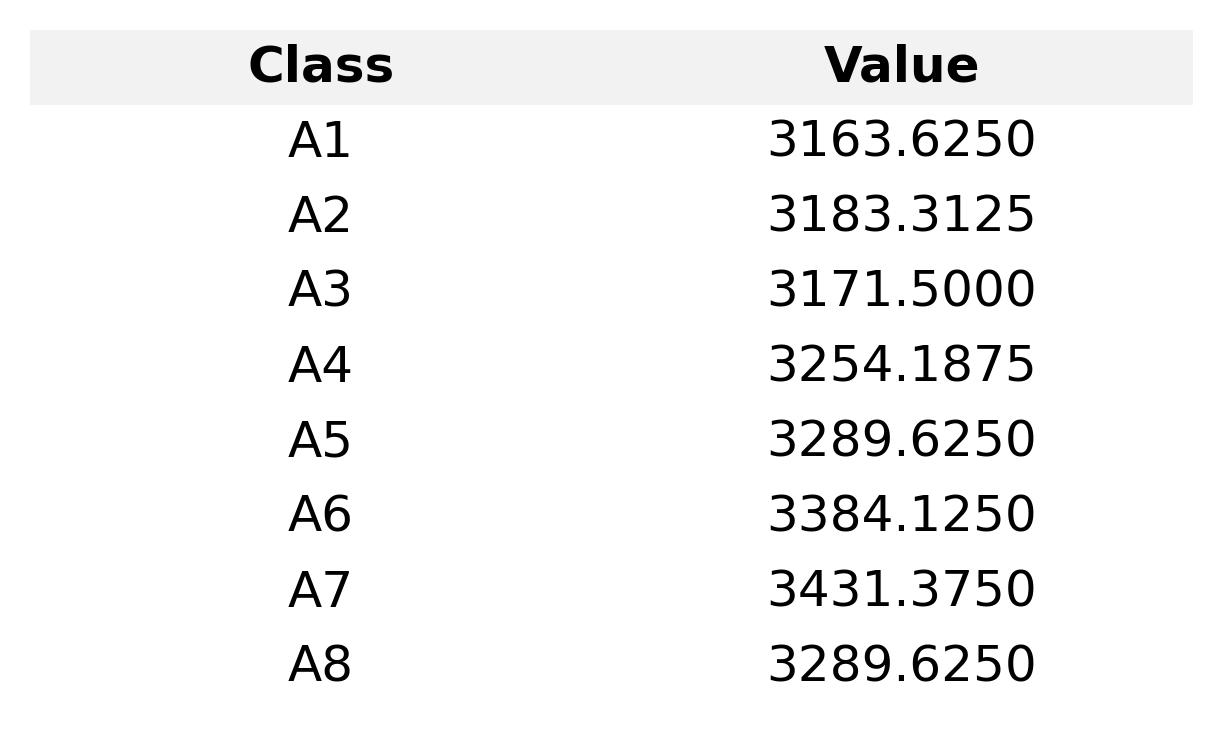
\includegraphics[scale=0.7]{images/flrg_table.jpg} 
    \caption{Fuzzy Logical Relationship Group}
\end{figure}

\subsection{\textit{Forecasting}}
Langkah terakhir adalah memasukkan data input ke dalam model FTS dan melakukan peramalan. Dengan menggunakan data historis dan nilai FLRG yang telah diperoleh, model FTS melakukan peramalan untuk memprediksi harga singkong di bulan selanjutnya. Berikut adalah contoh hasil peramalan harga singkong menggunakan model FTS:
\begin{figure}[H]
    \centering
    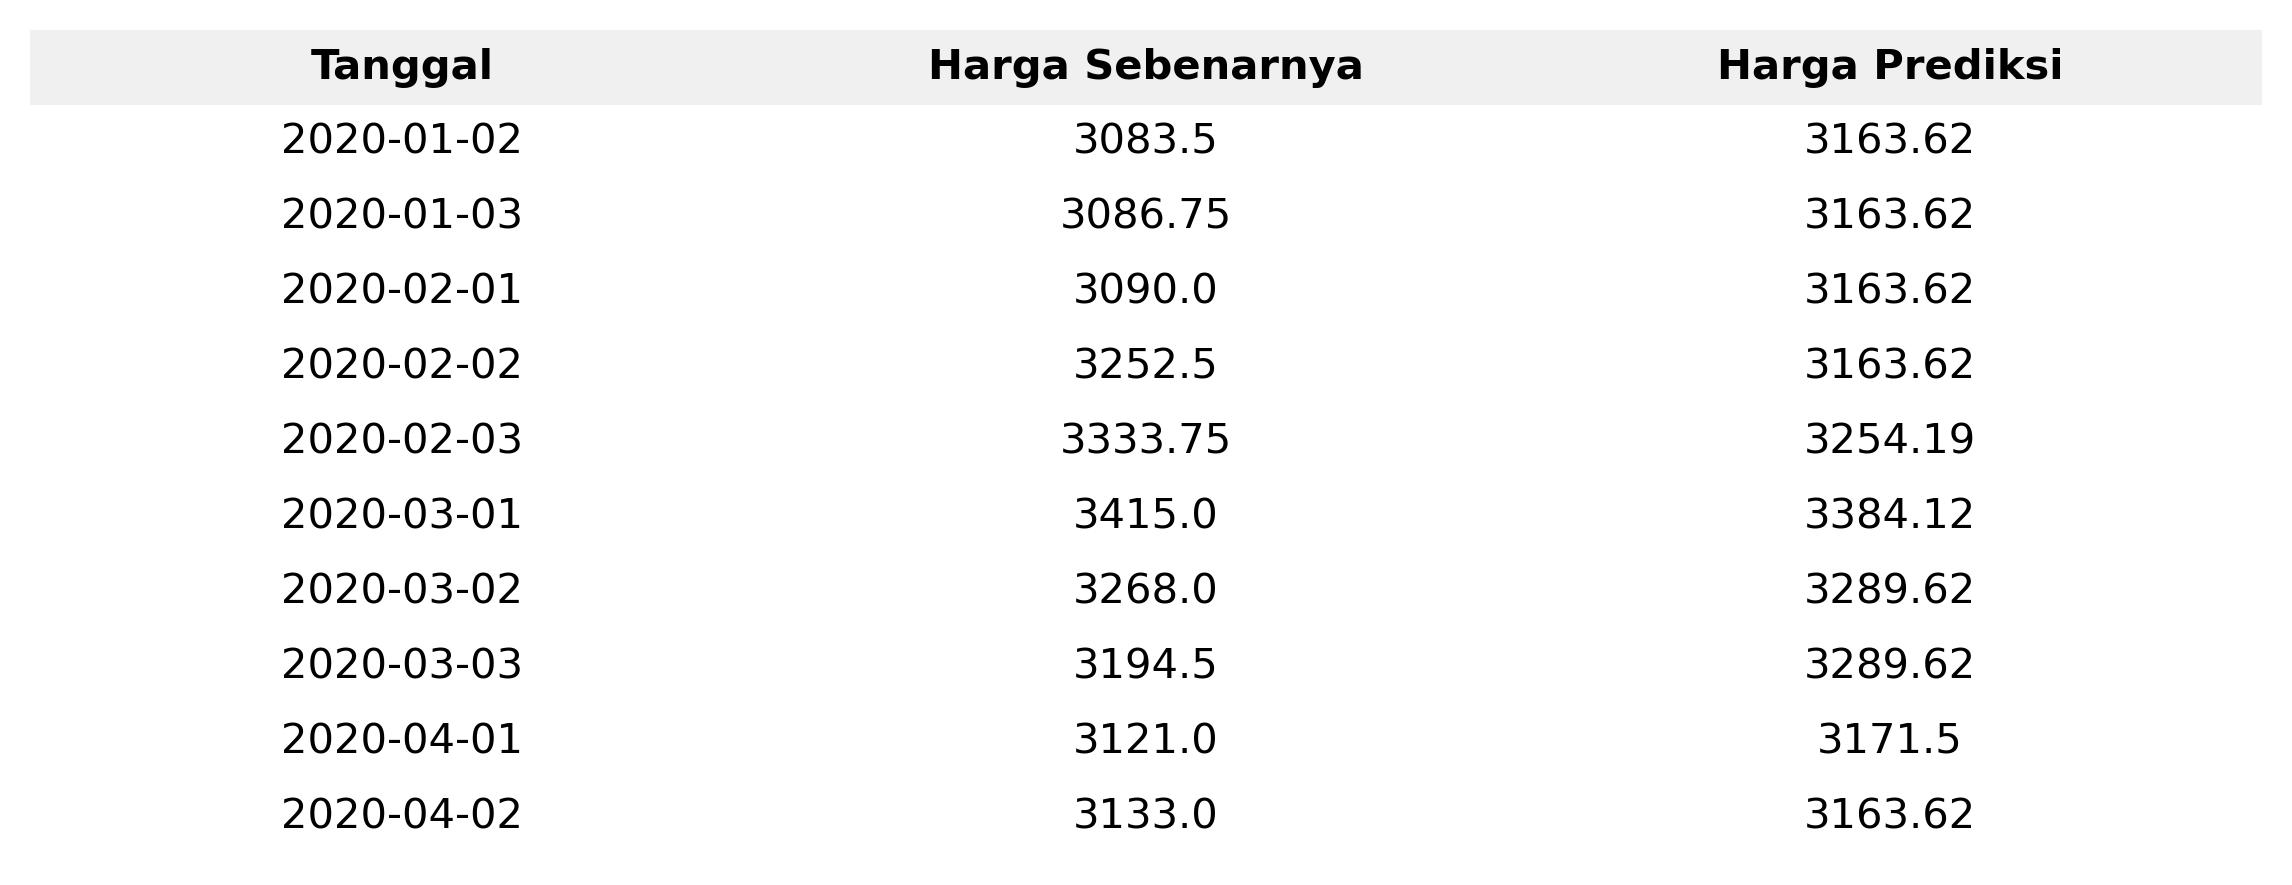
\includegraphics[scale=0.55]{images/tabel_perbandingan_harga.jpg} 
    \caption{Peramalan Harga Singkong}
\end{figure}


\subsection{Evaluasi model}
Evaluasi model dilakukan dengan membandingkan hasil peramalan dengan data aktual. Dalam evaluasi model data dibagi menjadi dua bagian, yaitu 70\% data training dan 30\% data testing. Dengan menggunakan metode \textit{Mean Absolute Percentage Error} (MAPE), dapat dihitung tingkat kesalahan peramalan. MAPE adalah metode yang digunakan untuk mengukur tingkat kesalahan peramalan dengan cara menghitung rata-rata persentase kesalahan peramalan. Rumus MAPE adalah sebagai berikut:
\begin{equation}
    MAPE = \frac{1}{n} \sum_{t=1}^{n} \left| \frac{A_t - F_t}{A_t} \right| \times 100\%
\end{equation}
dimana $A_t$ adalah data aktual, $F_t$ adalah data peramalan, dan $n$ adalah jumlah data. . Lalu untuk melakukan evaluasi model,  
Dengan menggunakan rumus tersebut, dapat dihitung tingkat kesalahan peramalan dan mengevaluasi model yang telah dibangun. Berdasarkan hasil evaluasi, model FTS dengan proporsi 70\% data training dan 30\% validasi memiliki tingkat kesalahan sebesar 1.26\% dan evaluasi model terhadap data validasi asli yaitu 2.01\% yang menunjukkan bahwa model ini cukup akurat berdasarkan hasil training.

\subsection{Pembahasan}
Metode \textit{fuzzy time series} (FTS) mungkin kurang cocok digunakan untuk memprediksi data yang memerlukan tingkat keakuratan dan ketelitian yang sangat tinggi. FTS bisa memprediksi sebuah harga barang untuk masa yang akan datang tetapi lebih bersifat klasifikasi, memperkirakan harga untuk bulan selanjutnya akan berada di class apa. Oleh karena itu, model FTS yang telah dibangun dalam penelitian ini dapat digunakan sebagai alat bantu untuk memprediksi harga singkong di bulan selanjutnya. Namun, model ini harus selalu diperbarui dengan data terbaru untuk mendapatkan hasil yang lebih akurat dan dapat diandalkan.



\begin{thebibliography}{00}
\bibitem{b1} Sarbaini, S., \& Yanti, D. (2023). Prediksi Harga Beras Belida Di Kota Pekanbaru Menggunakan Fuzzy Time Series Cheng. Jurnal Teknologi dan Manajemen Industri Terapan, 2(3), 234-241.
\bibitem{b2} Kementerian Pertanian. (2023). Pengaruh Perubahan Iklim Terhadap Sektor Pertanian. Upland.psp.pertanian.go.id. Diakses pada 15 Juni 2024, dari https://upland.psp.pertanian.go.id/public/artikel/1687919315/pengaruh-perubahan-iklim-terhadap-sektor-pertanian
\bibitem{b3} Ikhsanudin, A., Santoso, K. I., \& Wahyudion, S. (2022). Metode Fuzzy Time Series Model Chen untuk Memprediksi Jumlah Kasus Aktif Covid-19 di Indonesia. TRANSFORMASI, 18(1).
\bibitem{b4} Sumartini, S., Hayati, M. N., \& Wahyuningsih, S. (2017). Peramalan Menggunakan Metode Fuzzy Time Series Cheng. EKSPONENSIAL, 8(1), 51-56.
\bibitem{b5} Murni, C. K. (2023). Perbandingan Peramalan Penjualan Minuman Menggunakan Algoritma Single Exponential Smoothing Dan Triple Exponential Smoothing. Journal of Informatics Development, 1(2), 59-64.
\bibitem{b6} Ling, C.Y. Marques, J.A.L. (2024). Stock market prediction using artificial intelligence: A systematic review of systematic reviews, 9(1), 1-11. https://doi.org/10.1016/j.ssaho.2024.100864.
\bibitem{b7} Purwaningsih, S. S., Suryani, A., \& Taylor, A. (2015). PENGARUH INFLASI, SUKU BUNGA, DAN INDEKS HARGA SAHAM GABUNGAN (IHSG) TERHADAP KINERJA REKSADANA DENGAN PERMODELAN REGRESI DATA PANEL. Sigma-Mu, 7(2), 1-16.
\bibitem{b8} Wati, L., \& Solichin, A. (2024). Prediksi Nilai Pengadaan Barang Dan Jasa Pada Sebuah Perusahaan Pariwisata Menggunakan Metode Arima dan Fuzzy Time Series. Jurnal Inovtek Polbeng Seri Informatika, 9(1).
\bibitem{b9} Hablinawati, L., \& Nugraha, J. (2024). Peramalan Nilai Tukar Petani di Daerah Istimewa Yogyakarta Menggunakan Metode ARIMA: Peramalan Nilai Tukar Petani di Daerah Istimewa Yogyakarta Menggunakan Metode ARIMA. Emerging Statistics and Data Science Journal, 2(1).

\bibitem{b10} Nurlela, Siti, Fanani, Aris, \& Khaulasari, Hani (2023). Harga Minyak Mentah WTI Menggunakan Metode Fuzzy Time Series Markov Chain. Jurnal Fourier, 12(1), 10-19, ISSN 2541-5239, Al-Jamiah Research Centre, <https://doi.org/10.14421/fourier.2023.121.10-19>

\bibitem{b11} Song, Q., \& Chissom, B. S. (1993). Fuzzy time series and its models. Fuzzy sets and systems, 54(3), 269-277.

\bibitem{b12} Zhang, Y., \& Wu, L. (2009). Stock market prediction of S\&P 500 via combination of improved BCO approach and BP neural network. Expert systems with applications, 36(5), 8849-8854.

\bibitem{b13} Alptekin, D., Alptekin, B., \& Aladag, C. H. (2017). Forecasting Gold Prices with Fuzzy Time Series. Turkish Journal of Fuzzy Systems (TJFS), 8(2).

\bibitem{b14} Widarma, A., \& Siregar, Y. H. (2020). Sistem Prediksi Harga Produsen Padi Menggunakan Fuzzy Time Series. InfoTekJar: Jurnal Nasional Informatika dan Teknologi Jaringan, 5(1), 179-185.

\bibitem{b15} Vatansever, M., Demir, İ., \& Hepşen, A. (2020). Cluster and forecasting analysis of the residential market in Turkey: An autoregressive model-based fuzzy clustering approach. International Journal of Housing Markets and Analysis, 13(4), 583-600.


\end{thebibliography}

\end{document}